
% $Header: /cvsroot/latex-beamer/latex-beamer/solutions/conference-talks/conference-ornate-20min.en.tex,v 1.6 2004/10/07 20:53:08 tantau Exp $
\PassOptionsToPackage{pdfpagelabels=false}{hyperref}
\documentclass
%[handout] % Enable this opption if you want a compact printout of the talk for distribution.
{beamer}

% This file is a solution template for:

% - Talk at a conference/colloquium.
% - Talk length is about 20min.
% - Style is ornate.



% Copyright 2004 by Till Tantau <tantau@users.sourceforge.net>.
%
% In principle, this file can be redistributed and/or modified under
% the terms of the GNU Public License, version 2.
%
% However, this file is supposed to be a template to be modified
% for your own needs. For this reason, if you use this file as a
% template and not specifically distribute it as part of a another
% package/program, I grant the extra permission to freely copy and
% modify this file as you see fit and even to delete this copyright
% notice. 


\mode<presentation>
{
  \usetheme{Warsaw}
	\usecolortheme[RGB={0,102,51}]{structure}
  % or ...

  %\setbeamercovered{transparent}
  % or whatever (possibly just delete it)
}


\usepackage[english]{babel}
% or whatever

\usepackage[latin1]{inputenc}
% or whatever

\usepackage{times}
\usepackage[T1]{fontenc}
\usepackage{pgf,tikz}
\usepackage{color}
\usepackage{xcolor}
\usetikzlibrary{positioning}
%\usepackage{cases}

\def\mathunderline#1#2{\color{#1}\underline{{\color{black}#2}}\color{black}}
\usetikzlibrary{arrows}
\usetikzlibrary{calc}
\newcommand\scalemath[2]{\scalebox{#1}{\mbox{\ensuremath{\displaystyle #2}}}}
\newcommand{\R}{{\mathbb R}}
\newcommand{\Q}{{\mathbb Q}}
\newcommand{\C}{{\mathbb C}}
\newcommand{\N}{{\mathbb N}}
\newcommand{\Z}{{\mathbb Z}}
\newcommand{\Fr}{{\text{Fr}}}
\newcommand{\LCM}{\text{LCM}}
\newcommand{\multideg}{\text{multideg}}
\newcommand{\ord}{\text{ord}}
\newcommand{\Irr}{\text{Irr}}
% Or whatever. Note that the encoding and the font should match. If T1
% does not look nice, try deleting the line with the fontenc.

\definecolor{ffffff}{rgb}{1.0,1.0,1.0}
\definecolor{wwwwqq}{rgb}{0.4,0.4,0}
\definecolor{zzqqtt}{rgb}{0.6,0,0.2}
\definecolor{zzttqq}{rgb}{0.6,0.2,0}
\definecolor{qqwwcc}{rgb}{0,0.4,0.8}
\definecolor{fffftt}{rgb}{1,1,0.2}
\definecolor{qqqqff}{rgb}{0,0,1}
\definecolor{qqzzqq}{rgb}{0,0.6,0}
\definecolor{ffqqqq}{rgb}{1,0,0}
\definecolor{uququq}{rgb}{0.25,0.25,0.25}

\title[Basis] % (optional, use only with long paper titles)
{An Introduction to Resolving Sets and Metric Dimension}


%\author[McGuire] % (optional, use only with lots of authors)
%{Trevor McGuire}
% - Give the names in the same order as the appear in the paper.
% - Use the \inst{?} command only if the authors have different
%   affiliation.

\institute[NDSU] % (optional, but mostly needed)
{
  %
  Department of Mathematics\\
  North Dakota State University\\
  Fargo, ND}
  
% - Use the \inst command only if there are several affiliations.
% - Keep it simple, no one is interested in your street address.

%\date[AMS2007] % (optional, should be abbreviation of conference name)
%{Combinatorics Seminar, NDSU, September 2015}
% - Either use conference name or its abbreviation.
% - Not really informative to the audience, more for people (including
%   yourself) who are reading the slides online

 



% If you have a file called "university-logo-filename.xxx", where xxx
% is a graphic format that can be processed by latex or pdflatex,
% resp., then you can add a logo as follows:

% \pgfdeclareimage[height=0.5cm]{university-logo}{university-logo-filename}
% \logo{\pgfuseimage{university-logo}}



% Delete this, if you do not want the table of contents to pop up at
% the beginning of each subsection:



% If you wish to uncover everything in a step-wise fashion, uncomment
% the following command: 

%\beamerdefaultoverlayspecification{<+->}


\begin{document}

\begin{frame}
  \titlepage
\end{frame}

%\begin{frame}
  %\frametitle{Outline}
%  \tableofcontents
  % You might wish to add the option [pausesections]
%\end{frame}


% Structuring a talk is a difficult task and the following structure
% may not be suitable. Here are some rules that apply for this
% solution: 

% - Exactly two or three sections (other than the summary).
% - At *most* three subsections per section.
% - Talk about 30s to 2min per frame. So there should be between about
%   15 and 30 frames, all told.

% - A conference audience is likely to know very little of what you
%   are going to talk about. So *simplify*!
% - In a 20min talk, getting the main ideas across is hard
%   enough. Leave out details, even if it means being less precise than
%   you think necessary.
% - If you omit details that are vital to the proof/implementation,
%   just say so once. Everybody will be happy with that.
\section{Introduction}
\begin{frame}
  \frametitle{Representation of a node}
 \begin{definition}
     For an ordered subset $W=(w_1, w_2, ...)$ of vertices in $G$, the representation of a vertex $v \in G$ with respect to $W$ denoted $r(v/W)$ where $r:G\mapsto \mathbb{N}^{|W|}$ is defined by:
  \begin{align*}
  r(v/W)=(d(v,w_1), d(v,w_2), ...)
  \end{align*}
  Then $r(G/W)$ is the image of $r$ with respect to $W$ when applied to vertices in $G$.
\end{definition}
\end{frame}

\section{Bridge Subdivisions}



%\subsection{Background}
\begin{frame}
 \begin{center}
   \scalemath{.8}{
    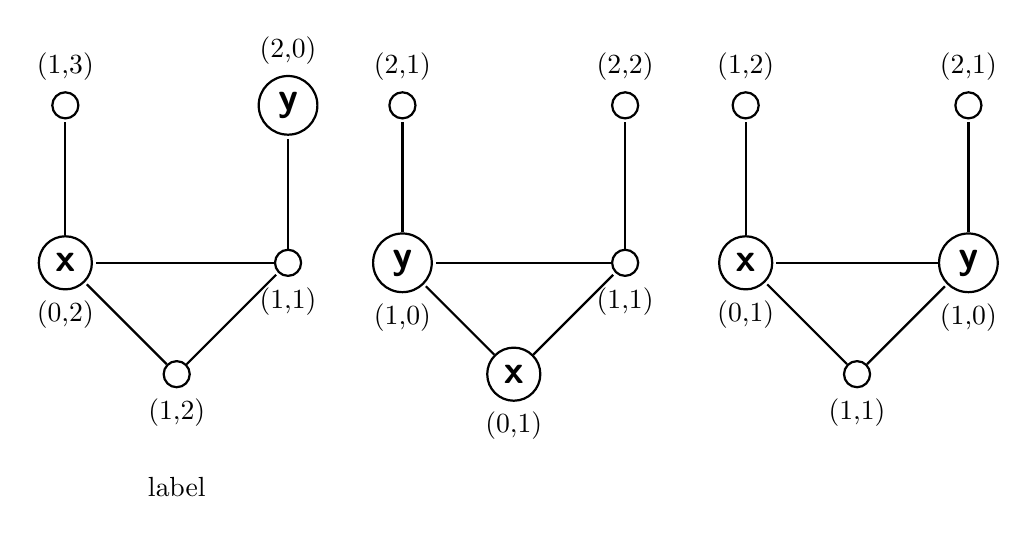
\begin{tikzpicture}[>=stealth',shorten >=1pt,auto, node distance=2cm,
                    thick,main node/.style={circle,draw,font=\sffamily\Large\bfseries}]
      \node[main node] (1) [label={270:(0,2)}] {x};
      \node[main node] (2) [below right of=1, label={270:(1,2)}]{};
      \node[main node] (3) [above right of=2, label={270:(1,1)}] {};
      \node[main node] (4) [above of=3, label={(2,0)}] {y};
      \node[main node] (5) [above of=1, label={(1,3)}] {};
      \node [below=1cm  of 2] {label};

      \path[thick]
	(2) edge (3)
	    edge (1)
	(3) edge (1)
	    edge (4)
	(1) edge (5);
      
      \node[main node] (6) [right= 3.75cm of 2,label={270: (0,1)}] {x};
      \node[main node] (7) [above right of=6, label={270:(1,1)}] {};
      \node[main node] (8) [above left of=6, label={270:(1,0)}] {y};
      \node[main node] (9) [above of=7, label={(2,2)}] {};
      \node[main node] (10) [above of=8, label={(2,1)}] {};

      \path[thick]
	(6) edge (7)
	    edge (8)
	(7) edge (8)
	    edge (9)
	(8) edge (10);


      \node[main node] (11) [right= 1cm of 7, label={270:(0,1)}] {x};
      \node[main node] (12) [below right of=11, label={270:(1,1)}]{};
      \node[main node] (13) [above right of=12, label={270:(1,0)}] {y};
      \node[main node] (14) [above of=13, label={(2,1)}] {};
      \node[main node] (15) [above of=11, label={(1,2)}] {};

      \path[thick]
	(12) edge (13)
	    edge (11)

	(13) edge (11)
	    edge (14)
	(11) edge (15);
	

    \end{tikzpicture}
  }
 \end{center}
\end{frame}

\begin{frame}
 \begin{center}
   \scalemath{.8}{
    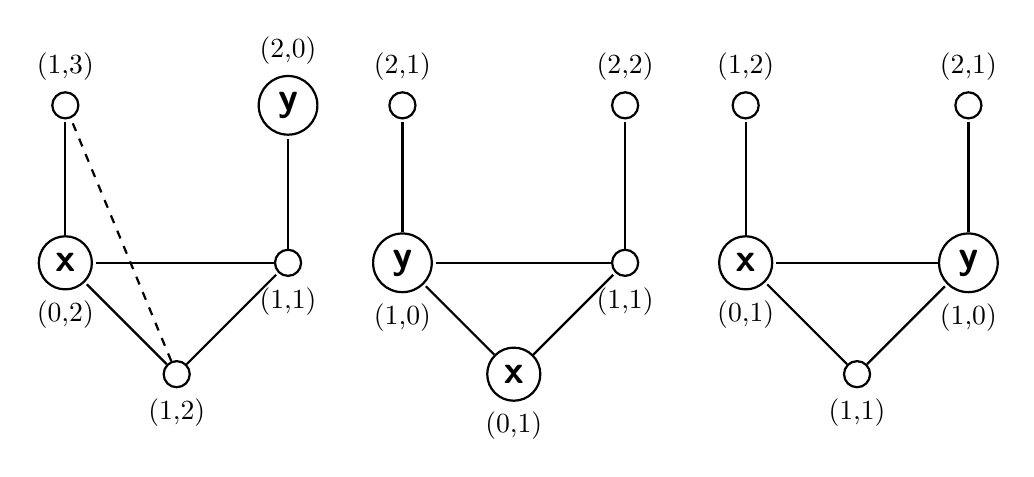
\begin{tikzpicture}[>=stealth',shorten >=1pt,auto, node distance=2cm,
                    thick,main node/.style={circle,draw,font=\sffamily\Large\bfseries}]
      \node[main node] (1) [label={270:(0,2)}] {x};
      \node[main node] (2) [below right of=1, label={270:(1,2)}]{};
      \node[main node] (3) [above right of=2, label={270:(1,1)}] {};
      \node[main node] (4) [above of=3, label={(2,0)}] {y};
      \node[main node] (5) [above of=1, label={(1,3)}] {};

      \path[thick]
	(2) edge (3)
	    edge (1)
	(3) edge (1)
	    edge (4)
	(1) edge (5);
      \path[thick]
      (2) edge [dashed] (5);
      
      \node[main node] (6) [right= 3.75cm of 2,label={270: (0,1)}] {x};
      \node[main node] (7) [above right of=6, label={270:(1,1)}] {};
      \node[main node] (8) [above left of=6, label={270:(1,0)}] {y};
      \node[main node] (9) [above of=7, label={(2,2)}] {};
      \node[main node] (10) [above of=8, label={(2,1)}] {};

      \path[thick]
	(6) edge (7)
	    edge (8)
	(7) edge (8)
	    edge (9)
	(8) edge (10);


      \node[main node] (11) [right= 1cm of 7, label={270:(0,1)}] {x};
      \node[main node] (12) [below right of=11, label={270:(1,1)}]{};
      \node[main node] (13) [above right of=12, label={270:(1,0)}] {y};
      \node[main node] (14) [above of=13, label={(2,1)}] {};
      \node[main node] (15) [above of=11, label={(1,2)}] {};

      \path[thick]
	(12) edge (13)
	    edge (11)

	(13) edge (11)
	    edge (14)
	(11) edge (15);
	
    \end{tikzpicture}
  }
 \end{center}
\end{frame}

\begin{frame}
 \begin{center}
   \scalemath{.8}{
    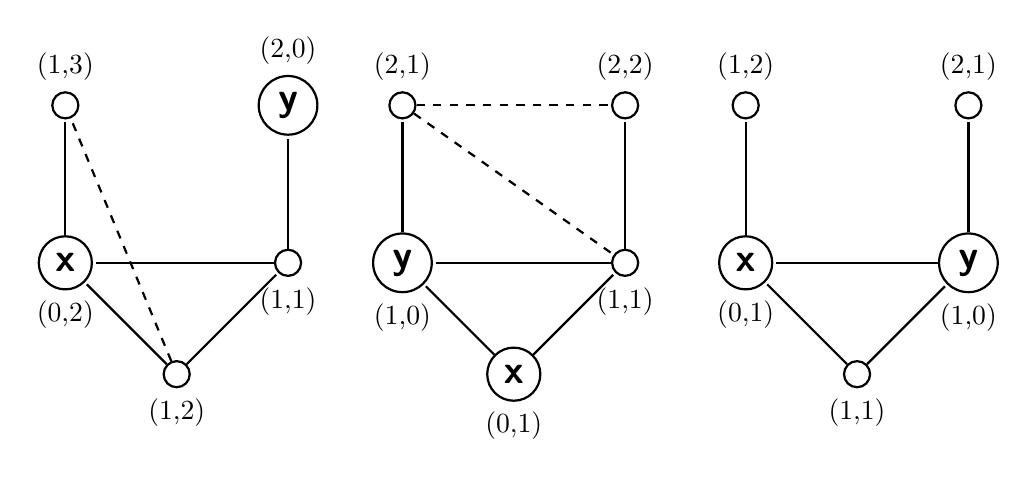
\begin{tikzpicture}[>=stealth',shorten >=1pt,auto, node distance=2cm,
                    thick,main node/.style={circle,draw,font=\sffamily\Large\bfseries}]
      \node[main node] (1) [label={270:(0,2)}] {x};
      \node[main node] (2) [below right of=1, label={270:(1,2)}]{};
      \node[main node] (3) [above right of=2, label={270:(1,1)}] {};
      \node[main node] (4) [above of=3, label={(2,0)}] {y};
      \node[main node] (5) [above of=1, label={(1,3)}] {};

      \path[thick]
	(2) edge (3)
	    edge (1)
	(3) edge (1)
	    edge (4)
	(1) edge (5);
      \path[thick]
      (2) edge [dashed] (5);
      
      \node[main node] (6) [right= 3.75cm of 2,label={270: (0,1)}] {x};
      \node[main node] (7) [above right of=6, label={270:(1,1)}] {};
      \node[main node] (8) [above left of=6, label={270:(1,0)}] {y};
      \node[main node] (9) [above of=7, label={(2,2)}] {};
      \node[main node] (10) [above of=8, label={(2,1)}] {};

      \path[thick]
	(6) edge (7)
	    edge (8)
	(7) edge (8)
	    edge (9)
	(8) edge (10);
      \path[thick]
	(10) edge [dashed] (7)
	    edge [dashed] (9);

      \node[main node] (11) [right= 1cm of 7, label={270:(0,1)}] {x};
      \node[main node] (12) [below right of=11, label={270:(1,1)}]{};
      \node[main node] (13) [above right of=12, label={270:(1,0)}] {y};
      \node[main node] (14) [above of=13, label={(2,1)}] {};
      \node[main node] (15) [above of=11, label={(1,2)}] {};

      \path[thick]
	(12) edge (13)
	    edge (11)

	(13) edge (11)
	    edge (14)
	(11) edge (15);

    \end{tikzpicture}
  }
 \end{center}
\end{frame}

\begin{frame}
 \begin{center}
   \scalemath{.8}{
    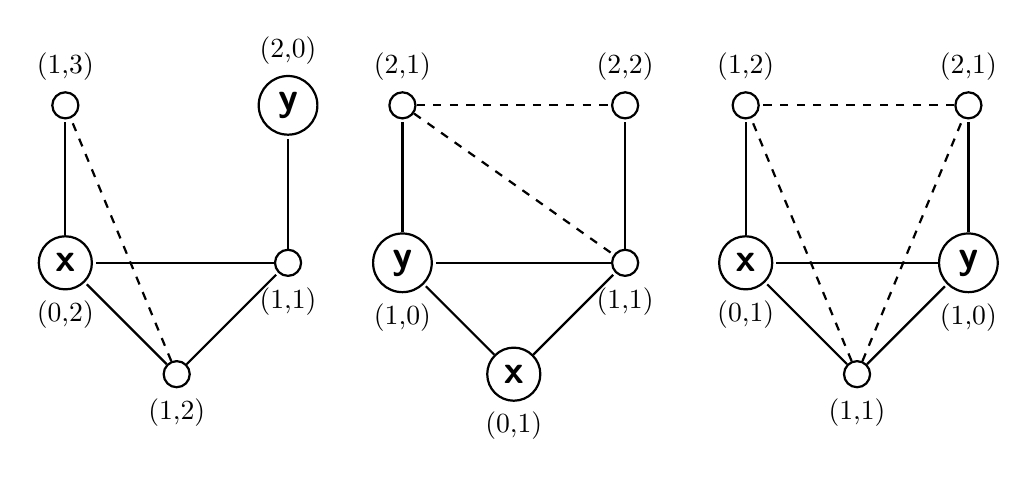
\begin{tikzpicture}[>=stealth',shorten >=1pt,auto, node distance=2cm,
                    thick,main node/.style={circle,draw,font=\sffamily\Large\bfseries}]
      \node[main node] (1) [label={270:(0,2)}] {x};
      \node[main node] (2) [below right of=1, label={270:(1,2)}]{};
      \node[main node] (3) [above right of=2, label={270:(1,1)}] {};
      \node[main node] (4) [above of=3, label={(2,0)}] {y};
      \node[main node] (5) [above of=1, label={(1,3)}] {};

      \path[thick]
	(2) edge (3)
	    edge (1)
	(3) edge (1)
	    edge (4)
	(1) edge (5);
      \path[thick]
      (2) edge [dashed] (5);
      
      \node[main node] (6) [right= 3.75cm of 2,label={270: (0,1)}] {x};
      \node[main node] (7) [above right of=6, label={270:(1,1)}] {};
      \node[main node] (8) [above left of=6, label={270:(1,0)}] {y};
      \node[main node] (9) [above of=7, label={(2,2)}] {};
      \node[main node] (10) [above of=8, label={(2,1)}] {};

      \path[thick]
	(6) edge (7)
	    edge (8)
	(7) edge (8)
	    edge (9)
	(8) edge (10);
      \path[thick]
	(10) edge [dashed] (7)
	    edge [dashed] (9);

      \node[main node] (11) [right= 1cm of 7, label={270:(0,1)}] {x};
      \node[main node] (12) [below right of=11, label={270:(1,1)}]{};
      \node[main node] (13) [above right of=12, label={270:(1,0)}] {y};
      \node[main node] (14) [above of=13, label={(2,1)}] {};
      \node[main node] (15) [above of=11, label={(1,2)}] {};

      \path[thick]
	(12) edge (13)
	    edge (11)

	(13) edge (11)
	    edge (14)
	(11) edge (15);
	
	\path[thick]
	(12) edge [dashed] (14)
	    edge [dashed] (15)
	(14) edge [dashed] (15);
    \end{tikzpicture}
  }
 \end{center}
\end{frame}



\begin{frame}

\begin{center}
\scalemath{.8}{
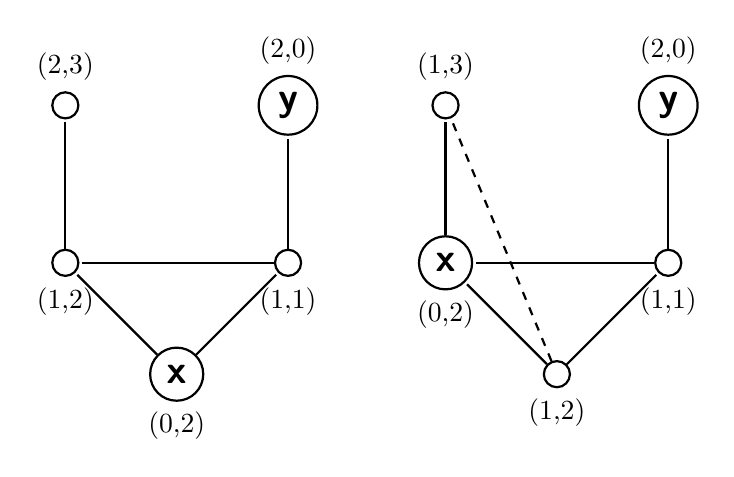
\begin{tikzpicture}[>=stealth',shorten >=1pt,auto, node distance=2cm,
                    thick,main node/.style={circle,draw,font=\sffamily\Large\bfseries}]
\node[main node] (1) [label={270: (0,2)}] {x};
\node[main node] (2) [above right of=1, label={270:(1,1)}] {};
\node[main node] (3) [above left of=1, label={270:(1,2)}] {};
\node[main node] (4) [above of=2, label={(2,0)}] {y};
\node[main node] (5) [above of=3, label={(2,3)}] {};

\path[thick]
  (1) edge (2)
      edge (3)
  (2) edge (3)
      edge (4)
  (3) edge (5);
  
\node[main node] (8) [right of=2, label={270:(0,2)}] {x};
\node[main node] (6) [below right of=8, label={270:(1,2)}]{};
\node[main node] (7) [above right of=6, label={270:(1,1)}] {};
\node[main node] (9) [above of=7, label={(2,0)}] {y};
\node[main node] (10) [above of=8, label={(1,3)}] {};

\path[thick]
  (6) edge (7)
      edge (8)
  (7) edge (8)
      edge (9)
  (8) edge (10);
\path[thick]
(6) edge [dashed] (10);
\end{tikzpicture}
}
\end{center}

\begin{center}
\scalemath{.8}{
 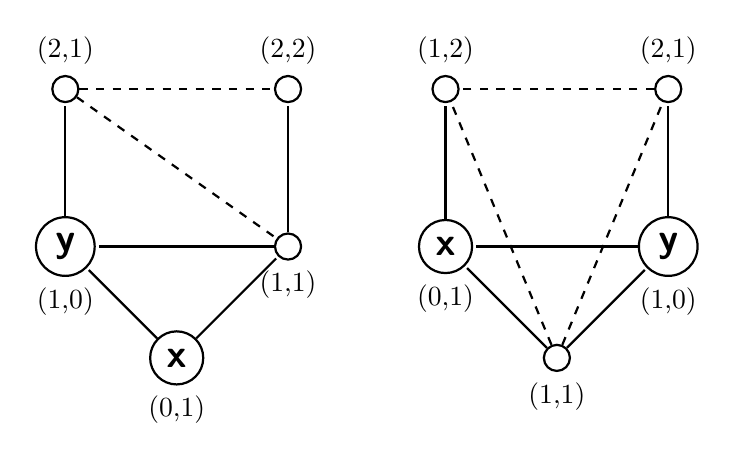
\begin{tikzpicture}[>=stealth',shorten >=1pt,auto,node distance=2cm,
                    thick,main node/.style={circle,draw,font=\sffamily\Large\bfseries}]
\node[main node] (1) [label={270: (0,1)}] {x};
\node[main node] (2) [above right of=1, label={270:(1,1)}] {};
\node[main node] (3) [above left of=1, label={270:(1,0)}] {y};
\node[main node] (4) [above of=2, label={(2,2)}] {};
\node[main node] (5) [above of=3, label={(2,1)}] {};

\path[thick]
  (1) edge (2)
      edge (3)
  (2) edge (3)
      edge (4)
  (3) edge (5);
\path[thick]
  (5) edge [dashed] (2)
      edge [dashed] (4);

\node[main node] (8) [right of=2, label={270:(0,1)}] {x};
\node[main node] (6) [below right of=8, label={270:(1,1)}]{};
\node[main node] (7) [above right of=6, label={270:(1,0)}] {y};
\node[main node] (9) [above of=7, label={(2,1)}] {};
\node[main node] (10) [above of=8, label={(1,2)}] {};

\path[thick]
  (6) edge (7)
      edge (8)

  (7) edge (8)
      edge (9)
  (8) edge (10);
  
  \path[thick]
  (6) edge [dashed] (9)
      edge [dashed] (10)
  (9) edge [dashed] (10);
\end{tikzpicture}
}
\end{center}
\end{frame}

\begin{frame}
\frametitle{Barbell Graph}
\begin{center}
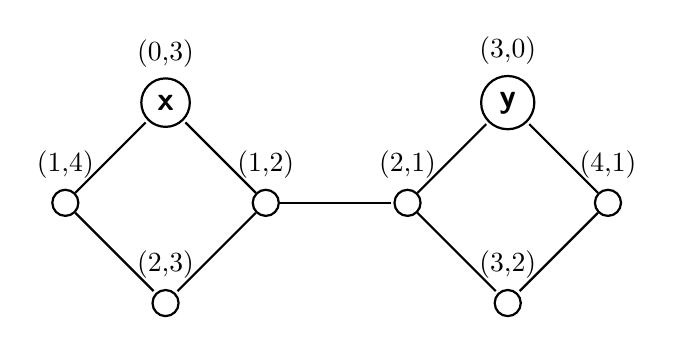
\begin{tikzpicture}[>=stealth',shorten >=1pt,auto,node distance=1.8cm,
                    thick,main node/.style={circle,draw,font=\sffamily\large\bfseries}]
\node[main node] (1) [label={(1,4)}] {};
\node[main node] (2) [above right of=1, label={(0,3)}] {x};
\node[main node] (3) [below right of=1, label={(2,3)}] {};
\node[main node] (4) [above right of=3, label={(1,2)}] {};
\node[main node] (5) [right of =4, label={(2,1)}] {};
\node[main node] (6) [above right of =5, label={(3,0)}] {y};
\node[main node] (7) [below right of =5, label={(3,2)}] {};
\node[main node] (8) [above right of =7, label={(4,1)}] {};

\path[thick]
  (1) edge (2)
      edge (3)
  (4) edge (2)
      edge (3)
      edge (5)
  (5) edge (6)
      edge (7)
  (8) edge (6)
      edge (7);

      
\end{tikzpicture}
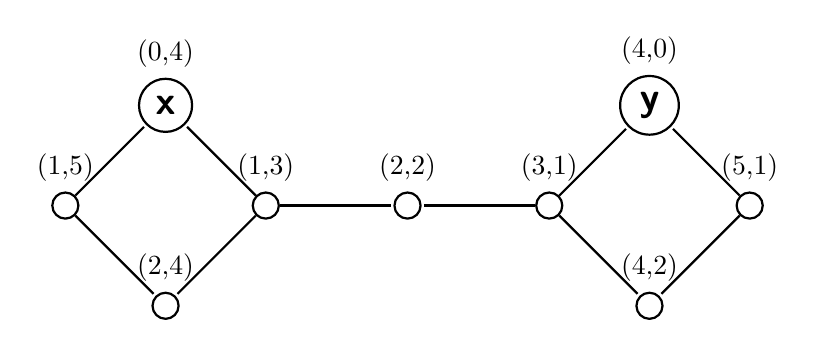
\begin{tikzpicture}[>=stealth',shorten >=1pt,auto,node distance=1.8cm,
                    thick,main node/.style={circle,draw,font=\sffamily\Large\bfseries}]
\node[main node] (1) [label={(1,5)}] {};
\node[main node] (2) [above right of=1, label={(0,4)}] {x};
\node[main node] (3) [below right of=1, label={(2,4)}] {};
\node[main node] (4) [above right of=3, label={(1,3)}] {};
\node[main node] (9) [right of =4, label={(2,2)}] {};
\node[main node] (5) [right of =9, label={(3,1)}] {};
\node[main node] (6) [above right of =5, label={(4,0)}] {y};
\node[main node] (7) [below right of =5, label={(4,2)}] {};
\node[main node] (8) [above right of =7, label={(5,1)}] {};


\path[thick]
  (1) edge (2)
      edge (3)
  (4) edge (2)
      edge (3)
      edge (9)
  (5) edge (6)
      edge (7)
      edge (9)
  (8) edge (6)
      edge (7);

      
\end{tikzpicture}

\end{center}

\end{frame}

\begin{frame}
\begin{center}
\LARGE Thank You!
\end{center}
\end{frame}
\end{document}


